\section{Fast Rotation}


\subsection{Generality}

The fast rotation refers to the cyclotron motion in the ring, which has a revolution frequency of 6.71 MHz (period of 149 ns) 
for muon propagating on the magic orbit with the magic momentum. 
The fast rotation signal corresponds to observing the evolution of the beam as it rotates around the ring. 
The transverse emittance of the beam and its momentum spread make the beam decohere (or debunch).
To understand how the momentum spread leads to decoherence, one have to remember that the orbit radius for a fixed magnetic
field is set by the momentum of the particle. Two particles injected on the magic orbit but with different momenta will
have different radii. Given than the speed of the muons almost does not depend on the momentum given they are relativistic,
the different momenta lead to different revolution frequencies. The higher momentum muon will complete a revolution
slower (larger radius) than the lower momentum muon (smaller radius). 
The small difference in revolution frequency leads to the beam having decohered after about 30 $\mu$s. 
From an initial beam with a limited longitudinal extension we end up with a beam filling entirely the ring.

\subsection{Analytical description}

FILL FIGURE FOR\newline
  * no  E spread, T spread\newline
  * add E spread\newline
  * add T spread\newline

Imagine that the initial muon distribution has zero emittance (no transverse size), zero momentum spread and zero bunch length (no longitudinal extension). 
The particles share a common revolution period $T$ and the time dependence of the intensity signal at a fixed point (signal measured with a fiber harp for example), is 

\begin{equation}
I(t)=\delta\left(t-\left(n+\frac{\theta}{2\pi}\right)T\right),
\end{equation} 
where $n$ is any non negative integer that corresponds to the number of revolution in the ring, 
and $\theta$ is the azimuthal position of the point in the ring.
Figure~\ref{fig:perfect_frs} shows what the fast rotation signal looks like for a beam with characteristics described above.
The beam remains unchanged as a function of time given its perfectness.

\begin{figure}[bt]
\centering
\subfigure[]{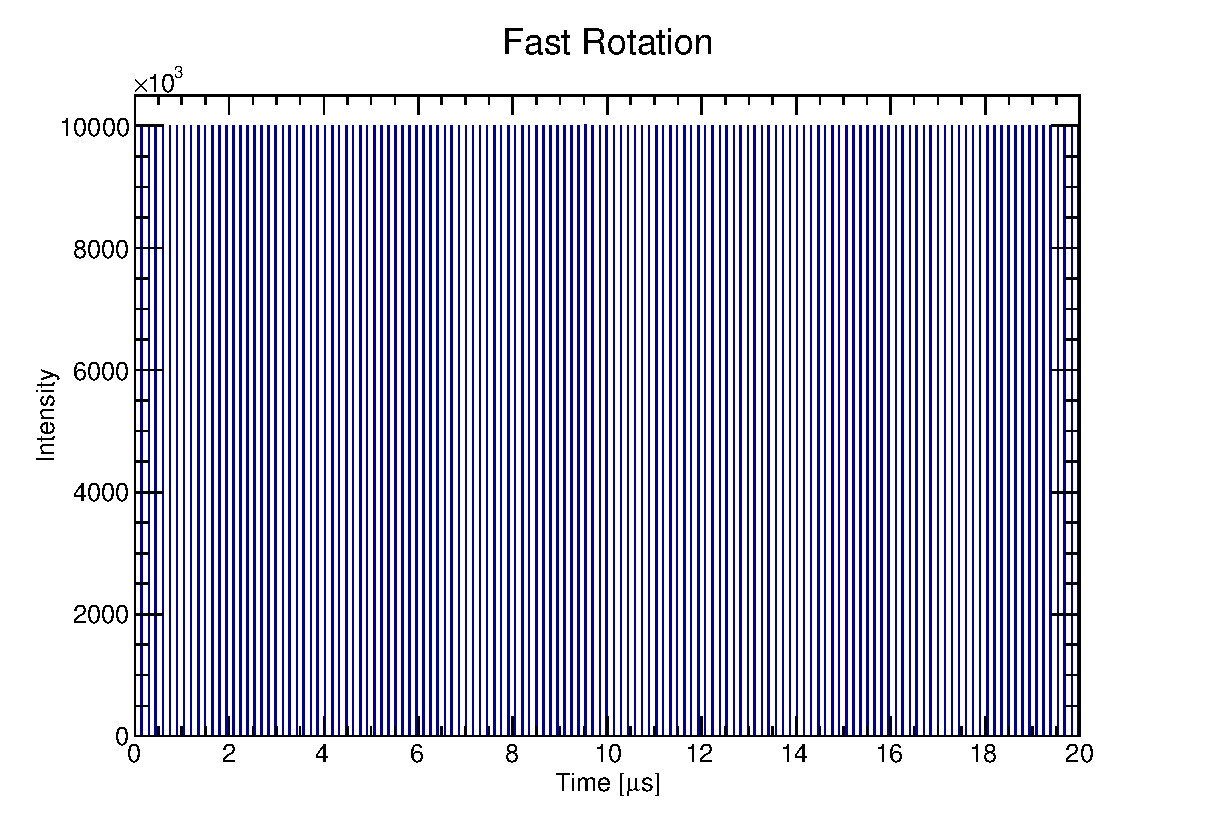
\includegraphics[width=0.45\textwidth]{fig/FRS_noSpread_0-20_us.eps}}
\subfigure[]{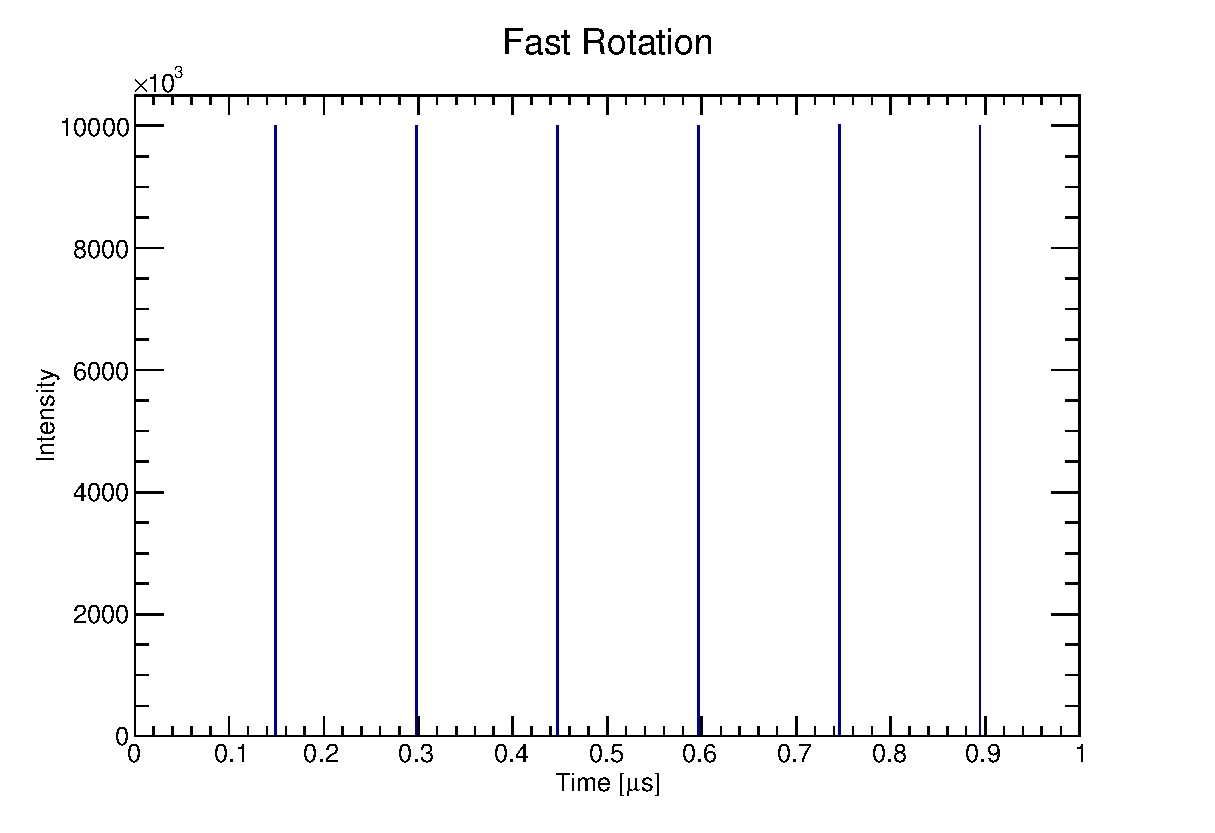
\includegraphics[width=0.45\textwidth]{fig/FRS_noSpread_0-1_us.eps}}
\caption{Fast rotation signal as a function of time for a muon beam with zero emittance, zero momentum spread and zero bunch length.}
\label{fig:perfect_frs}
\end{figure}
 
A particle with momentum offset $\Delta$ will have revolution period $T(1+\Delta)$, so that 
\begin{equation}
I(t,\Delta)=\delta\left(t-\left(n+\frac{\theta}{2\pi}\right)T\left(1+\Delta\right)\right). 
\end{equation}
The fast rotation signal at the point is then~\footnote{the notation $(n+\frac{\theta}{2\pi})T$ will be noted thereafter $nT$ for improved text clarity} 

\begin{equation}
S(t)=\sum^{\infty}_{n=0}\int\rho(\Delta)\delta\left(t-nT\left(1+\Delta\right)\right)d\Delta 
\end{equation}
where $\rho(\Delta)$ is the distribution of momenta offsets. If the momentum distribution is a Gaussian with width $\Delta_0$, then 

\begin{eqnarray}
S(t) &=& \sum^{\infty}_{n=0}\int\frac{e^{-\Delta^2/(2\Delta^2_0)}}{\sqrt{2\pi}\Delta_0}
\delta\left(t-nT\left(1+\Delta\right)\right)d\Delta\\
&=&\sum^{\infty}_{n=0}\int\frac{e^{-\Delta^2/(2\Delta^2_0)}}{\sqrt{2\pi}\Delta_0}\frac{\delta\left(\Delta-\left(\frac{t}{nT}-1\right)\right)}{nT}d\Delta\\
&=&\sum^{\infty}_{n=0}\frac{e^{-(\frac{t}{nT}-1)^2/2\Delta^2_0}}{\sqrt{2\pi}\Delta_0nT}\label{eq:Espread_frs}
%&=&\sum^{\infty}_{n=0}\frac{e^{-(t-nT)^2/2\Delta^2_0(n+\theta/2\pi)^2T^2}}{\sqrt{2\pi}\Delta_0nT}\label{eq:Espread_frs}
\end{eqnarray}

Note that there is no muon decay in Eq.~(\ref{eq:Espread_frs}) or the accompanying plots.
Figure~\ref{fig:Espread_frs} shows the fast rotation signal for a beam with zero emittance, zero bunch length but with a 0.112\% momentum spread. 
One can see that the beam decoheres. The decoherence envelope is set by the momentum spread, the more spread the faster the decoherence.

\begin{figure}[bt]
\centering
\subfigure[]{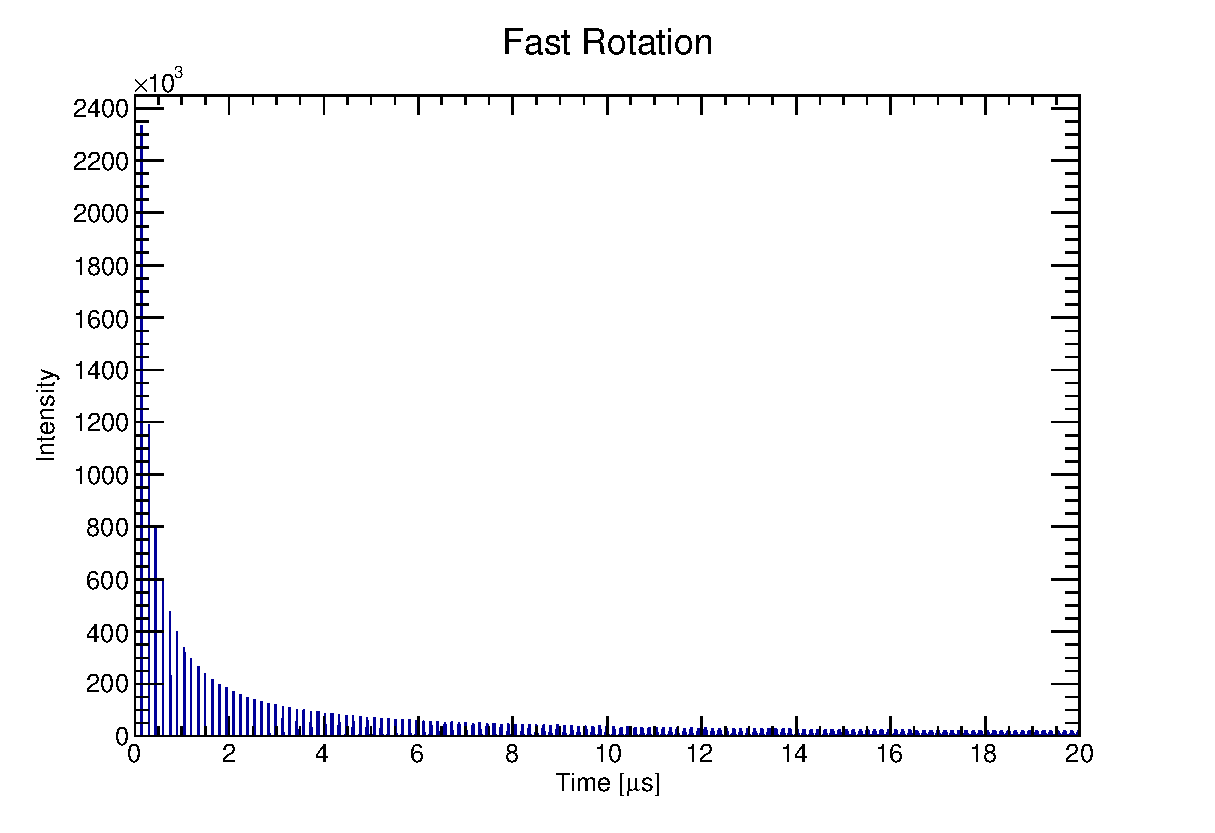
\includegraphics[width=0.6\textwidth]{fig/FRS_pSpread112_0-20us.eps}}\\
\subfigure[]{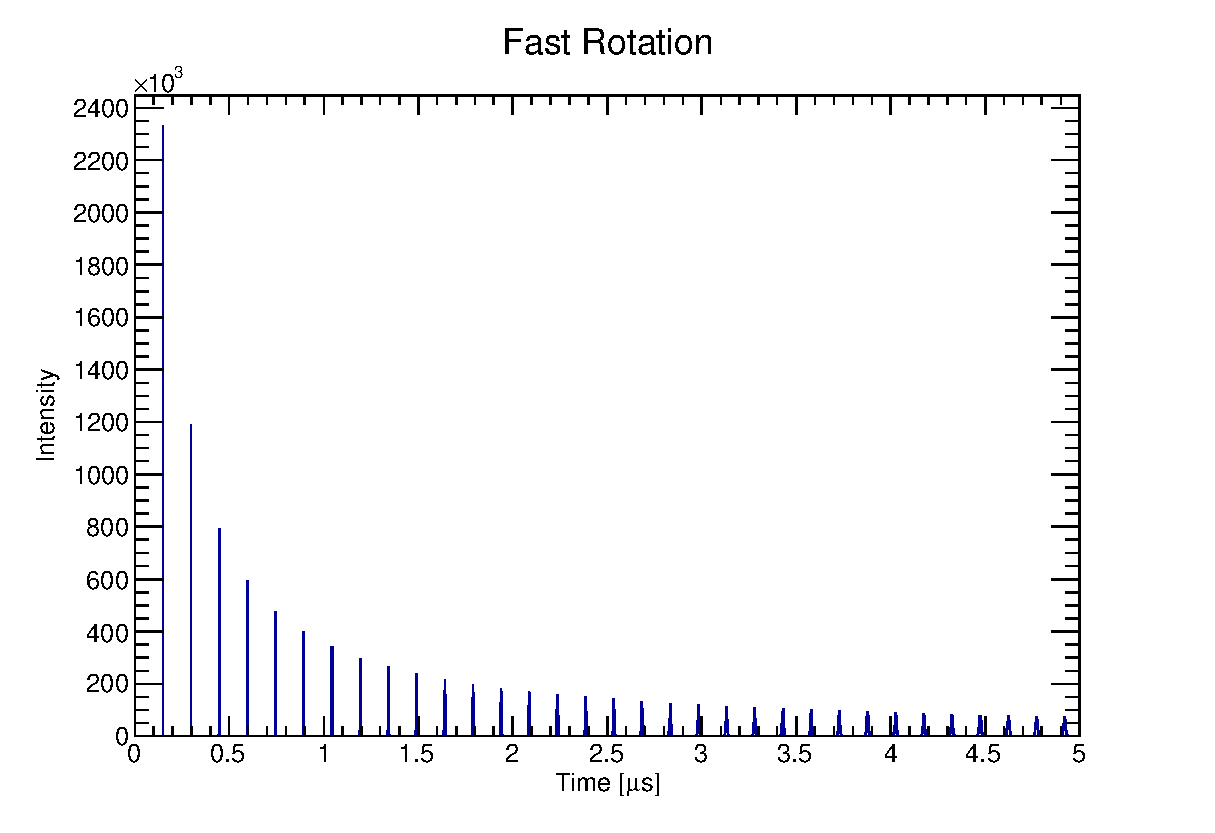
\includegraphics[width=0.45\textwidth]{fig/FRS_pSpread112_0-5us.eps}}
\subfigure[]{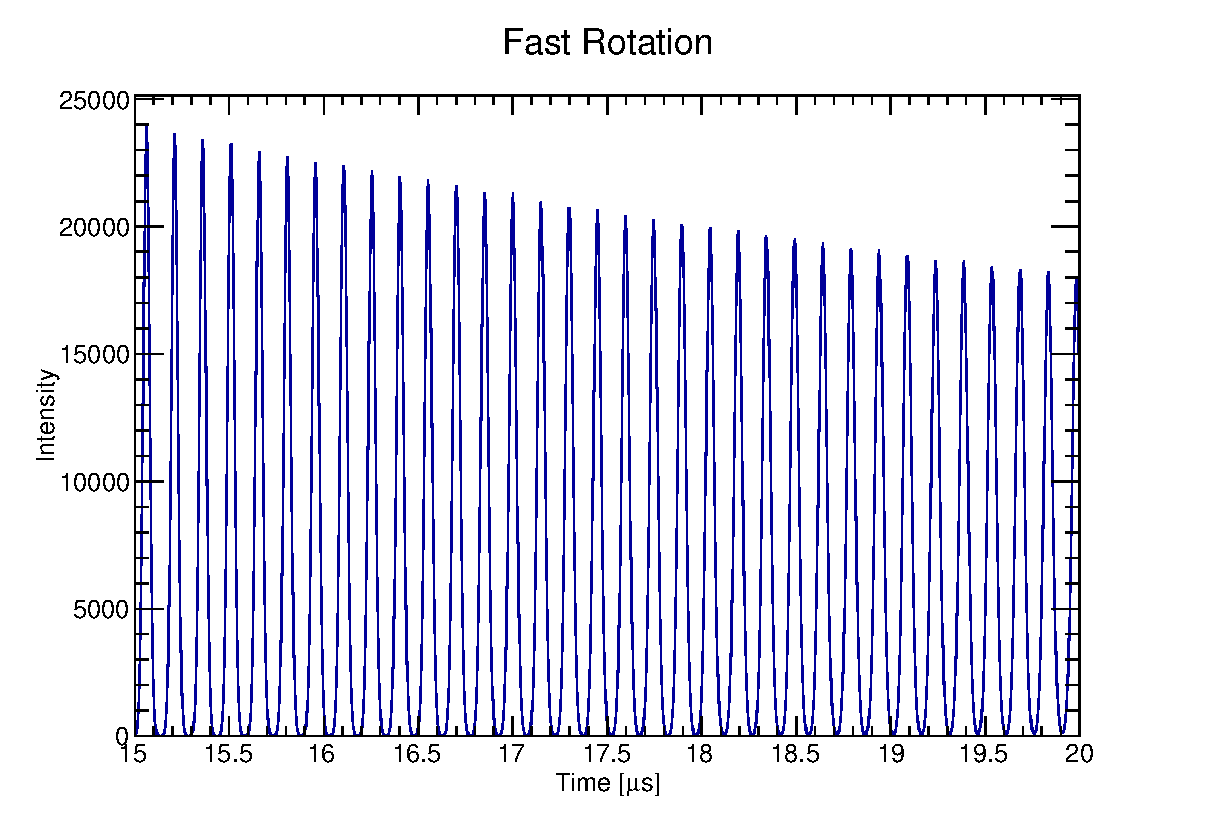
\includegraphics[width=0.45\textwidth]{fig/FRS_pSpread112_15-20us.eps}}
\caption{Fast rotation signal as a function of time for a muon beam with zero emittance, zero bunch length but width a 0.112\% momentum spread.}
\label{fig:Espread_frs}
\end{figure}

A realistic beam has on top of the momentum spread a non-zero bunch length. 
In this case Eq.~(\ref{eq:Espread_frs}) is re-expressed introducing a temporal offset $t^\prime$ as

\begin{eqnarray}
S(t,t^{\prime})&=& \sum_{n=0}^\infty\frac{e^{-(\frac{t-t^\prime}{nT}-1)^2/(2\Delta_0^2)}}{\sqrt{2\pi}\Delta_0 nT}
\end{eqnarray}

Suppose the intial temporal (longitudinal) distribution of the muons is Gaussian $$\xi(t^\prime) = \frac{1}{\sqrt{2\pi}\sigma_t}e^{-{t^\prime}^2/(2\sigma_t^2)}$$
Then
{\small
\begin{eqnarray*}
S(t)&=& \sum_{n=0}^\infty\int_{-\infty}^\infty dt^\prime \frac{e^{-(\frac{t-t^\prime}{nT}-1)^2/(2\Delta_0^2)}}{\sqrt{2\pi}\Delta_0 nT}\frac{1}{\sqrt{2\pi}\sigma_t}e^{-{t^\prime}^2/(2\sigma_t^2)}
\\
&=& \sum_{n=0}^\infty\frac{1}{2\pi\Delta_0nT\sigma_t}\int_{-\infty}^\infty dt^\prime e^{-(\frac{t-t^\prime}{nT}-1)^2/(2\Delta_0^2)}e^{-{t^\prime}^2/(2\sigma_t^2)}\\
%&=& \sum_{n=0}^\infty\frac{1}{2\pi\Delta_0(n+theta/2\pi)T\sigma_t}e^{-t^2/(2((n+theta/2\pi)T\Delta_0)^2)}
%\int_{-\infty}^\infty dt^\prime e^{-(\frac{{t^\prime}^2-2t t^\prime}{(nT)^2}+1 -\frac{2(t-t^\prime)}{nT})/(2\Delta_0^2)}e^{-{t^\prime}^2/(2\sigma_t^2)}\\
&=& \sum_{n=0}^\infty\frac{1}{2\pi\Delta_0nT\sigma_t}e^{-t^2/(2(nT\Delta_0)^2)}
\int_{-\infty}^\infty dt^\prime e^{-(\frac{{t^\prime}^2-2t t^\prime}{(nT)^2}+1 -\frac{2(t-t^\prime)}{nT})/(2\Delta_0^2)}e^{-{t^\prime}^2/(2\sigma_t^2)}\\
&=&\sum_{n=0}^\infty\frac{1}{2\pi\Delta_0nT\sigma_t}e^{-t^2/(2(nT\Delta_0)^2)}e^{\frac{t}{nT\Delta_0^2}}
\int_{-\infty}^\infty dt^\prime \exp(-{t^\prime}^2(\frac{1}{2(nT)^2\Delta_0^2}+\frac{1}{2\sigma_t^2})+t^\prime(\frac{t}{nT}-1)/(nT\Delta_0^2))e^{-1/(2\Delta_0^2)}\\
&=&\sum_{n=0}^\infty\frac{1}{2\pi\Delta_0nT\sigma_t}e^{-(\frac{t}{nT}-1)^2/2\Delta_0^2}
\int_{-\infty}^\infty dt^\prime \exp\left(-\alpha {t^\prime}^2+\beta t^\prime\right)\\
&=&\sum_{n=0}^\infty\frac{1}{2\pi\Delta_0nT\sigma_t}e^{-(\frac{t}{nT}-1)^2/(2\Delta_0^2)}
\sqrt{\frac{\pi}{\alpha}}e^{\beta^2/4\alpha}
\end{eqnarray*}
}
where $\alpha = \frac{1}{2(nT)^2\Delta_0^2}+\frac{1}{2\sigma_t^2}$ and $\beta= (\frac{t}{nT}-1)/(nT\Delta_0^2)$.
Finally
{\small
\begin{eqnarray}
S(t)&=&\sum_{n=0}^\infty\frac{1}{2\pi\Delta_0nT\sigma_t}e^{-(\frac{t}{nT}-1)^2/(2\Delta_0^2)}
\frac{\sqrt{2\pi}nT\Delta_0\sigma_t}{\sqrt{(nT)^2\Delta_0^2+\sigma_t^2}}
\exp(\frac{(\frac{t}{nT}-1)^2}{(nT\Delta_0^2)^2}\frac{(nT)^2\Delta_0^2\sigma_t^2}{2(nT)^2\Delta_0^2+2\sigma_t^2})\nonumber\\
&=& \frac{1}{\sqrt{2\pi}}\sum_{n=0}^\infty e^{-(\frac{t}{nT}-1)^2/(2\Delta_0^2)}
\frac{1}{\sqrt{((nT)^2\Delta_0^2+\sigma_t^2}}
\exp(\frac{(\frac{t}{nT}-1)^2}{\Delta_0^2}\frac{\sigma_t^2}{2(nT)^2\Delta_0^2+2\sigma_t^2})\nonumber\\
&=& \frac{1}{\sqrt{2\pi}}\sum_{n=0}^\infty
\frac{1}{\sqrt{((nT)^2\Delta_0^2+\sigma_t^2}}
\exp(\frac{-(\frac{t}{nT}-1)^2}{2\Delta_0^2}\left(1-\frac{\sigma_t^2}{(nT)^2\Delta_0^2+\sigma_t^2}\right))\label{eq:frs-sigt}
\end{eqnarray}
}


Figure~\ref{fig:E_T_spread_frs} shows the fast rotation signal for a beam with zero emittance, non-zero bunch length and non-zero momentum spread.
One can see that the beam decoheres faster having a longitudinal extension. It is expected since the longitudinal extension can be seen as 
created by a beam with an momentum spread having undergone an arbitrary number of revolution.

\begin{figure}[bt]
\centering
\subfigure[]{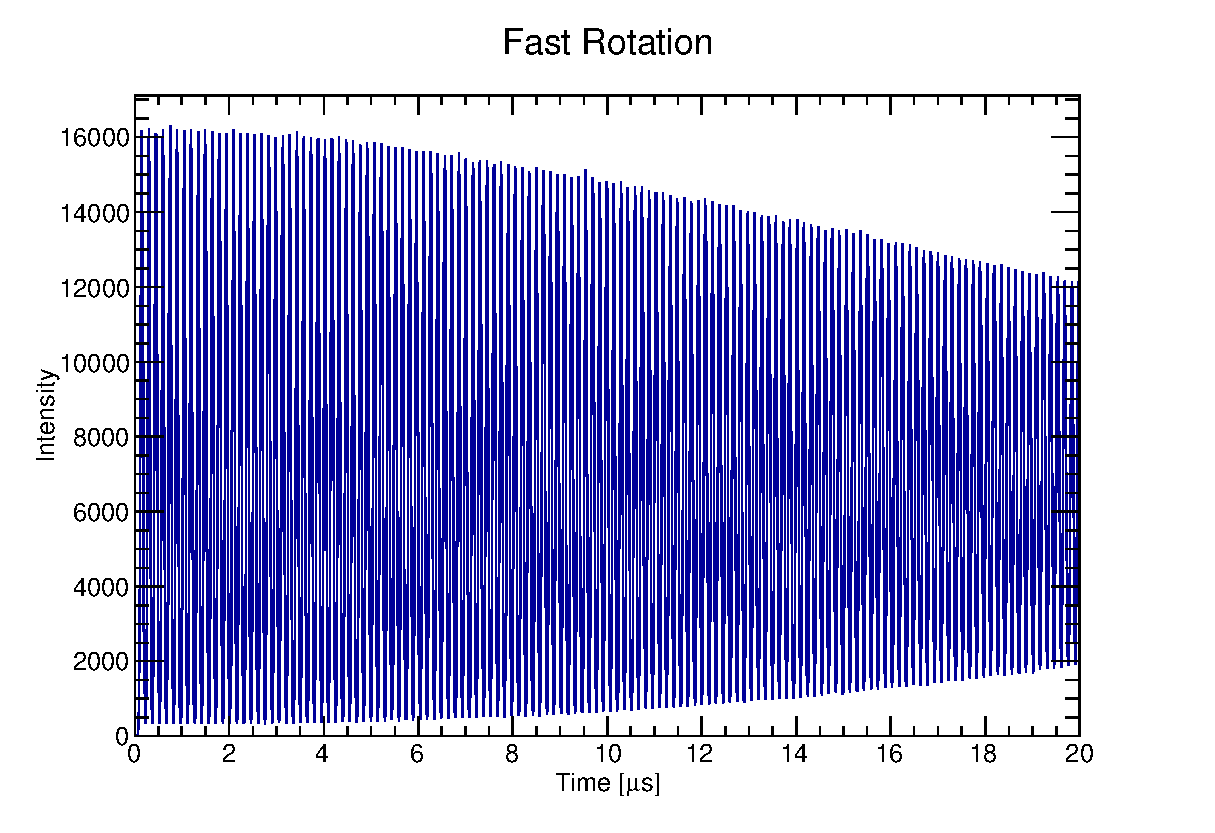
\includegraphics[width=0.6\textwidth]{fig/FRS_pSpread112_tSpread25ns_0-20us.eps}}\\
\subfigure[]{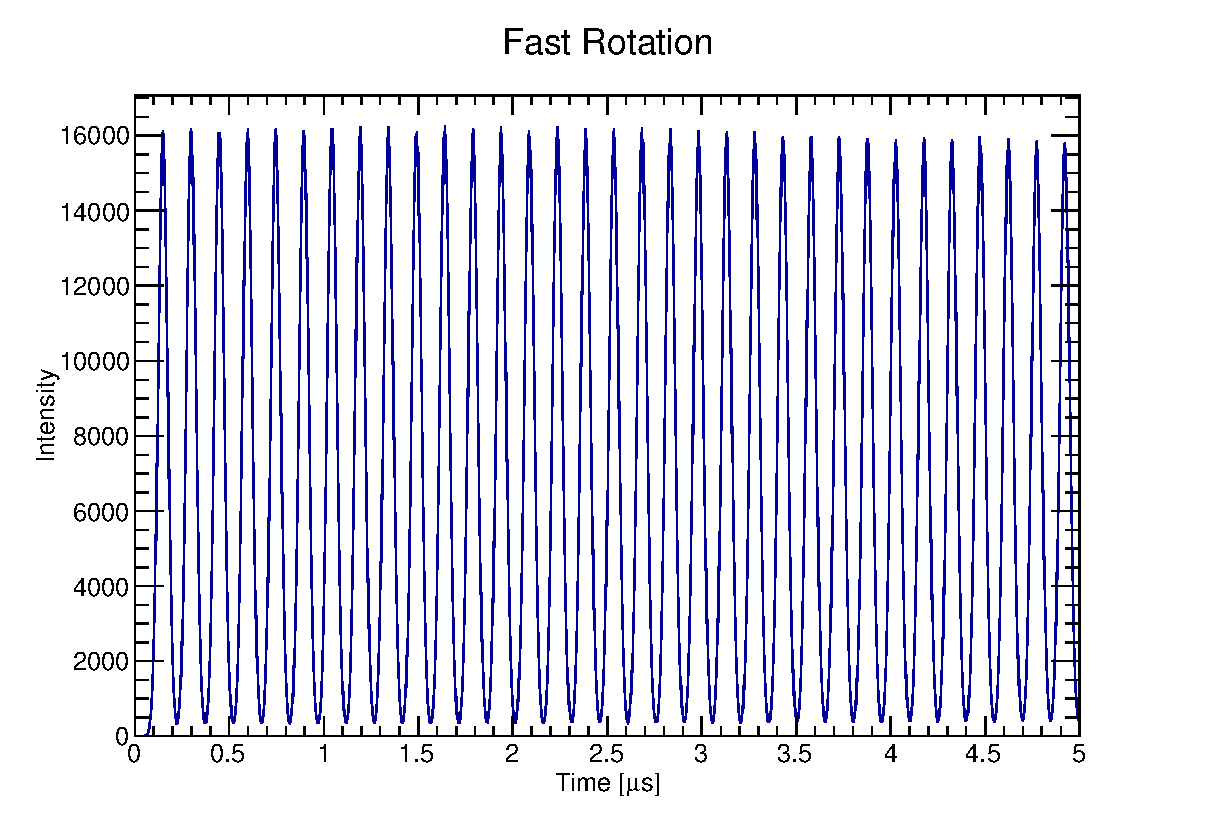
\includegraphics[width=0.45\textwidth]{fig/FRS_pSpread112_tSpread25ns_0-5us.eps}}
\subfigure[]{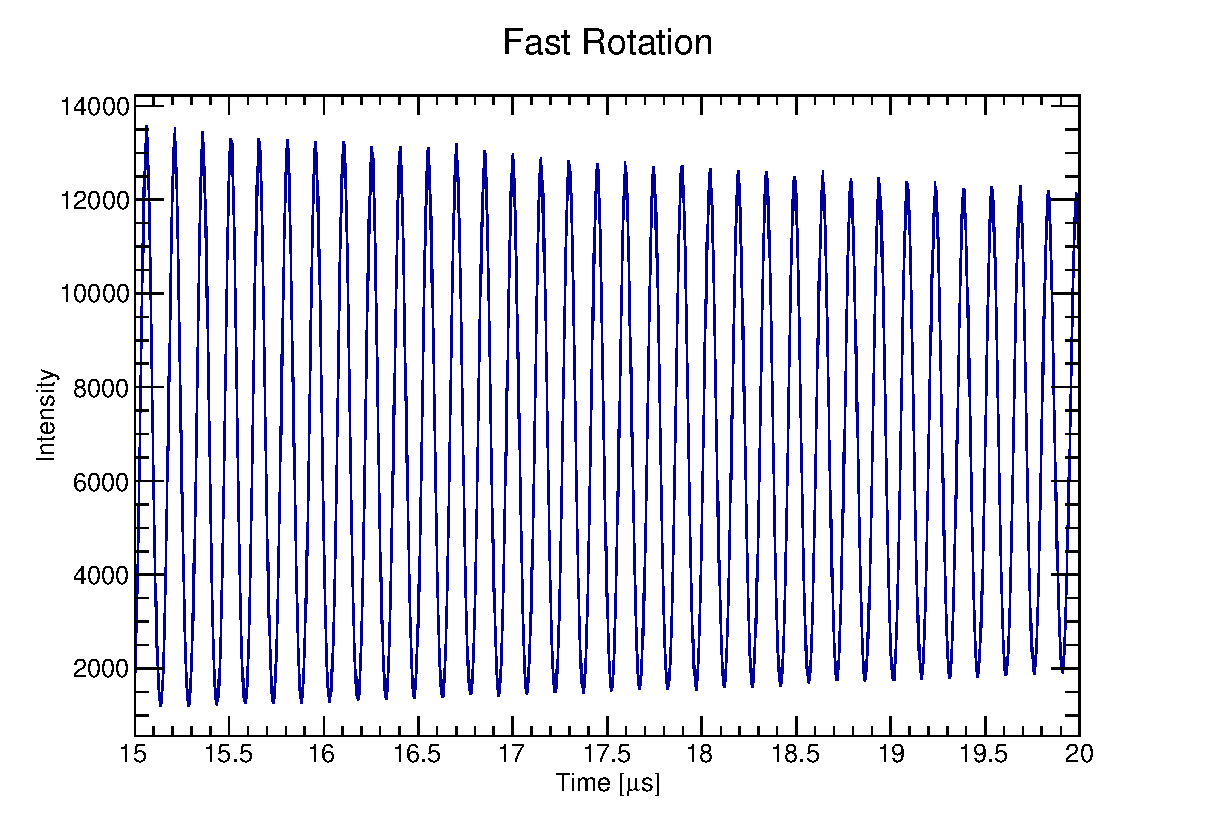
\includegraphics[width=0.45\textwidth]{fig/FRS_pSpread112_tSpread25ns_15-20us.eps}}
\caption{Fast rotation signal as a function of time for a muon beam with zero emittance, bunch length of 20 ns and momentum spread of 0.112\%.}
\label{fig:E_T_spread_frs}
\end{figure}
